\chapter{Annotation Service}

\section{Objective of the Annotation Service}
As described in 2.4.2, the goal of the AS is to provide a user with the possibility to:
\begin{enumerate}[(1)]
	\item view A WSI
	\item annotate a WSI
	\item manage made annotations
\end{enumerate}

In order to achieve objective (1) - (3), a GUI needs to be deployed which supports the user in working on those tasks. (3) also adds the need for file persistence management.


\section{Methodology}
As stated in 2.1, most vendors have proprietary image formats and their own implementation of a viewer for those, thus creating a vendor lock-in. Further do vendors often only support Windows platforms, ignoring other operating systems\cite{Cornish13}\cite{DICOM10}\cite{Farahanil15}. To avoid this, a solution must be found that is independent of operating system and vendor.

Chap. 3 already established a service to convert WSIs of various formats into the DZI format, solving the problem of multiple proprietary formats. 

Independence from an operating system can be achieved by using web technologies, especially when running an application in a web browser\cite{Tseytlin14}, since those are supported by all modern operating systems. 

Because of this, the AS will be implemented as a web browser application. 


\subsection{Functionality of the Annotation Service}
The goal of viewing a WSI (1) is a straight forward task. (2) and (3) are more elusive. For that reason, this subsection elaborates on the functionality needed to help achieve those objectives.

Annotations will be created by drawing directly onto the viewed WSI. If the user spots a region of interest, a contour can be drawn around it. This can  either be done in \emph{free hand} or \emph{polygon mode}. In free hand mode, the contour will be drawn along the path of the mouse pointer, until the mode is disabled again. Upon deactivation, the contour will be closed. In polygon mode, the user can place coordinates which will be connected from one to another in the order they're placed in. A contour in this mode considers to be closed, once a point on the contour is clicked a second time. A marked region of interest is simply called \emph{region} from this point on.

The information what a region is surrounded by can be as valuable as the information about the region itself\cite{Bankman00}. Therefore, every region will have a \emph{context} trait, which lists every label of regions it touches, crosses, surrounds or is surrounded by (see fig. \ref{fig4_contextregions}).

\begin{figure}[H]
	\begin{center}
		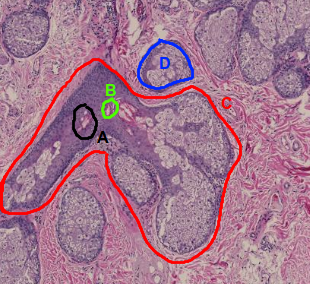
\includegraphics[scale=0.8]{img/contextregions.png}
		\caption{Example of context regions (B, C are context of A; A, C are context of B; A, B are context of C; D has no context region)}
		\label{fig4_contextregions}
	\end{center}
\end{figure}
% TODO: add figure about context regions

Another way of creating regions will be so called \emph{points of interest} (POI)\nmc{POI}{Point of Interest}. A POI will be placed with a mouse click. After that, an external script will be invoked to run an automated segmentation in the proximity of the POI and return with a contour which will be marked as region. The segmentation approaches may differ drastically in different scenarios\cite{Liu12}, therefore the script will be interchangeable\footnote{There are many different ways of how to approach the topic of segmentation (e.g. \cite{Qi12}, \cite{Sharma16}, \cite{Wienert12}, \cite{Angulo10} for cell segmentation alone). Writing a fully working segmentation script is worth another thesis by itself, therefore only a dummy implementation will be delivered with this work.}.

Each region has a \emph{label} associated to it. A label is a predefined string, which describes what the region just created shows. The labels available will be determined through a \emph{label dictionary}, which is a container that offers a list of strings to select from. This approach guarantees a unified labeling, independent of a specific WSI or pathologist. The option to choose between multiple available label dictionaries opens up the possibility of creating dictionaries which are specialized on certain cases or studies. Again, to keep up labeling integrity, labels can only be selected from one dictionary per WSI.

Users will be able to create new, empty dictionaries, if the need arises. Furthermore, they will be able to add entries to existing and new dictionaries alike, to further advance or specialize them. To delete single entries or whole dictionaries, file access to the server is necessary. This is due to the fact, that knowledge can by added without direct negative consequences. Deleting existing knowledge influences all WSIs on which this knowledge was used, may it be as a label or a whole dictionary.

To support the user in annotating a WSI, a distance measurement tool will be usable as well. This tool can measure the distance between 2 pixels in $\mu$m.


\subsection{Parts of the Annotation Service}
The AS is implemented in 2 parts. Those are the Annotation Service Server (ASS)\nmc{ASS}{Annoation Service Server} and the Annotation Service Viewer (ASV)\nmc{ASV}{Annotation Service Viewer}.

This is because of the \emph{same-origin policy} (SOP)\nmc{SOP}{same-origin policy}. SOP is a security concept of the web application security model. It prevents a direct access to files, if the parent directory of the originating file is not an ancestor directory of the target file\cite{web:mdn}. Because of the SOP, WSIs would have to be located in the directory structure of the AS, which by itself doesn't create a problem. To get a new WSI there, however, the user would be forced to navigate through the structure of the AS, find the correct directory and then place it there manually. This makes knowledge of the service structure necessary and creates a horrible UX. Furthermore, tinkering with the file structure of the AS creates a possible source for errors.

A workaround of this problem is to deploy a web server, which can redirect the image request, access the WSI and return it in response\cite{Tseytlin14}. The use of DZI creates another advantage: the used image pyramid model reduces the network traffic necessary to load and show a WSI in a viewer\cite{Cornish13}\cite{DICOM10}.

Furthermore, even a single WSI takes up a lot of storage capacity\cite{Singh11}. Having multiple WSIs on a local hard drive would either create the need for huge amounts of available storage space or restrict the amount of accessible WSIs to a few at any given time. The latter solution would create two follow-up problems:
\begin{itemize}
	\item WSIs are medical images and as such confidential information. Therefore, not everyone is allowed to just have access to or copies of them\cite{COA}\cite{USSanDiego}. Once a copy of a WSI changes hands, it is virtually impossible to make sure that privacy regulations will be uphold.	
	\item With only a small amount out of all WSIs accessible at all times, the need for copying files back and forth arises as soon as the user wants to compare, update or correct a WSI, which is not on his local file system at the given moment. Not only is this a great source for possible errors, but also very time consuming and inefficient.
\end{itemize}

With the use of a web server as a central image repository, WSIs and the access to them can be managed in a centralized spot, while upholding confidentiality regulations. Furthermore, a user has access to all of her/his WSIs at any given time, without the need for creating subsets and copying files back and forth. Depending on the setup of the network, other factors can come into play as well. Access to and sharing of rare cases, educational material and training samples can be granted without a complicated distribution chain and a smaller risk for confidentiality issues. It also enables the consultation of case experts independent of their physical position on the planet\cite{Wilbur09}.


\subsubsection{Annotation Service Server}
The ASS has 2 main purposes.

First, it serves as a so called \emph{Digital Slide Repository} (DSR)\nmc{DSR}{Digital Slide Repository}. A DSR manages storage of WSIs and their metadata. Furthermore, it serves requested image data to a viewer client, such as the ASV\cite{Cornish13}. 

Second, it is responsible for file management. In detail, this means:
\begin{itemize}
	\item persist made annotations in a file
	\item deliver annotation data together with image data
	\item serve list of all available label dictionaries
	\item serve label dictionary entries
	\item save added entries to existing label dictionary
	\item create new label dictionaries
\end{itemize}




% local for now


\subsubsection{Annotation Service Viewer}
To enable the pathologist to view a WSI and annotate it, a GUI needs to be deployed. This GUI will be called Annotation Service Viewer and developed in an iterative approach with the help of selected pathologists. After each iteration, the GUI and user experience (UX)\nmc{UX}{User Experience} will be evaluated. This way, the ASV can be adapted to the needs of a real life environment based on the pathologists feedback.

\begin{figure}[H]
	\begin{center}
		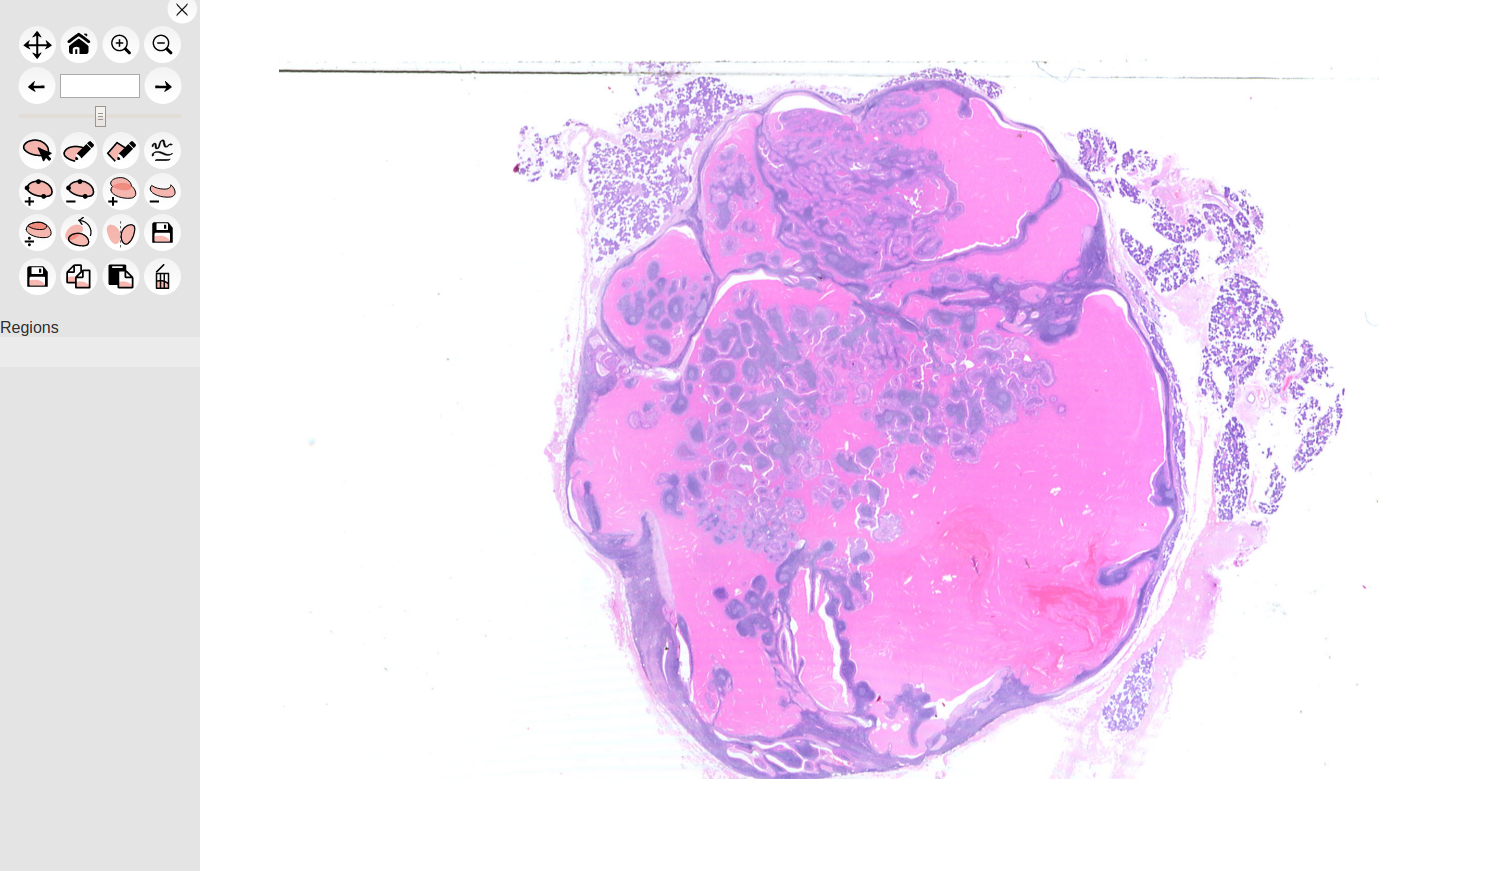
\includegraphics[scale=0.2]{img/microdrawUI.png}
		\caption{Microdraw GUI with opened WSI}
		\label{fig4_microdrawUI}
	\end{center}
\end{figure}

The first iteration of the ASV will be based on an open source project called \emph{MicroDraw}\footnote{See \url{https://github.com/r03ert0/microdraw} for more information on the MicroDraw project} (see fig. \ref{fig4_microdrawUI} for MicroDraws GUI).  MicroDraw is a web application to view and annotate \emph{"high resolution histology data"}\cite{web:microdraw2}. The visualization is based on another open source project, called \emph{OpenSeadragon}\cite{web:openseadragon}. Annotations are made possible by the use of \emph{Paper.js}\footnote{see \url{http://paperjs.org/} for more information on Paper.js}. Apart from the frameworks used, MicroDraw is written in JavaScript using HTML5, CSS3 and jQuery\footnote{see \url{https://jquery.com/} for more information on jQuery}.


\section{Implementation}
% what was used for implementation
\subsection{Technologies and Frameworks}
% openslide, openslide web server
% python web server, flask, openslide, java script, html5, css, jquery
\subsection{Annotation Service Viewer}
% documentation
\subsection{Annotation Service Server}
% documentation